\section{design of CoIncGraph}
\label{sec:design}

%  这一段还要重点修改一下，现在和最新的还没对应上

Figure~\ref{fig:1} presents an overview of CoIncGraph, a CPU--GPU cooperative system for incremental processing of streaming graphs that exceed GPU memory capacity. CoIncGraph integrates two components. First, a heterogeneous graph organization localizes adjacency changes and associated maintenance to modified source vertices. A unified change view coordinates updates to outgoing adjacency, the reverse index, and GPU views, avoiding redundant maintenance across these structures (Section~\ref{sec:graph-organization}). Second, a two-phase incremental execution pipeline performs deletion repair followed by insertion propagation. Compact worklists identify affected vertices: the CPU prepares incoming edges for GPU-based repair, while the GPU propagates improvements through outgoing edges (Section~\ref{sec:incremental-computation}). Together, these components confine data preparation and traversal to affected states and their dependencies, reducing redundant computation and CPU--GPU communication. In addition, CoIncGraph incorporates workload-specific optimizations to improve performance and broaden its applicability across diverse graph workloads (Section~\ref{sec:workload-cost}).

% We present a CPU--GPU cooperative system for out-of-memory streaming graph processing (Fig.~\ref{fig:1}). Section~\ref{sec:graph-organization}introduces a heterogeneous graph organization that confines adjacency changes and corresponding updates on the GPU and elsewhere to modified source vertices. A unified change view coordinates outgoing adjacency, the reverse index, and GPU views, reducing redundant maintenance across these structures. Building on this organization, Section~\ref{sec:incremental-computation} develops two-phase incremental computation: deletion repair followed by insertion propagation. Compact work lists identify affected vertices, guiding CPU preparation of incoming edges for GPU repair and GPU traversal from vertices whose results improve. This cooperation restricts data preparation and graph traversal to the affected computation and its dependencies, reducing redundant computation and CPU--GPU communication.

\begin{figure}[t]
\centering
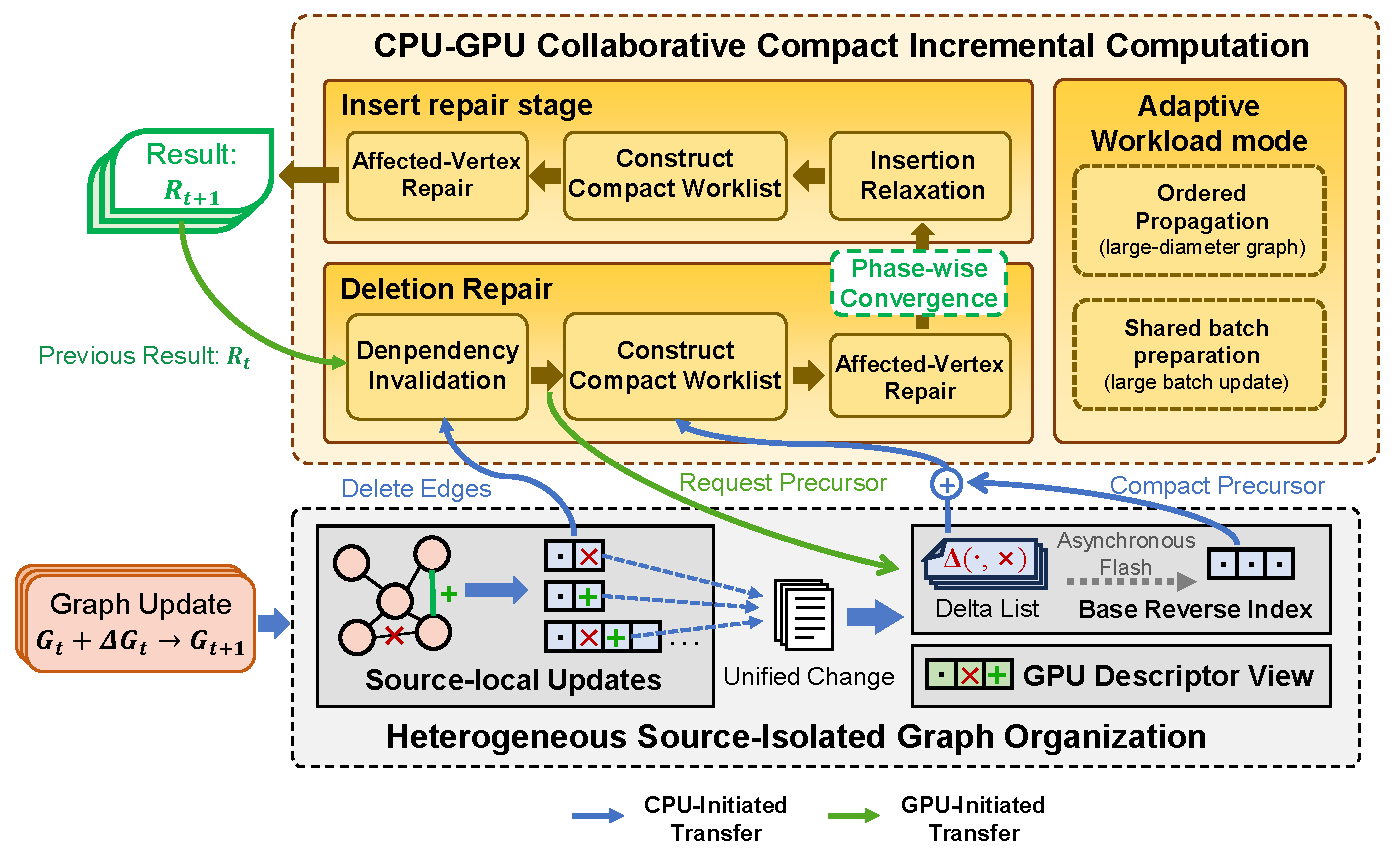
\includegraphics[width=\columnwidth]{figures/Overview.pdf}
\caption{The Overview of CoIncGraph System.}
\label{fig:1}
\end{figure}

\subsection{Heterogeneous Source-Isolated Graph Organization}
\label{sec:graph-organization}

Section~\ref{sec:motivation} shows that shared-array layouts transform a local update into the relocation of unrelated sources, resulting in extensive descriptor modifications and per-batch cache reorganization. The key idea of our graph organization is to \textit{make the source vertex of an update edge the unit of storage, change description, and GPU publication}, so that maintenance cost follows the set of changed sources rather than the graph size. It consists of three mechanisms. \textit{Source-isolated adjacency blocks} allocate each source's adjacency independently, so that an update never relocates other sources. A \textit{unified change view} resolves each batch once into effective edge changes and changed sources that drive all graph views. \textit{Coordinated view maintenance} uses this view to update the reverse index, publish GPU descriptors, and repair cached adjacency only for changed sources.

% Topological locality offers an opportunity to limit adjacency movement and GPU index maintenance to the sources whose outgoing adjacency changes in a batch. However, insertion operations in the PMA structure may trigger rebalancing, causing the adjacency list to be migrated to a locality other than that of the source vertex, thereby increasing the volume of data movement and the overhead of index maintenance at other locations. We organize maintenance around independently allocated source blocks. Section 4.1 explains how this layout prevents updates from relocating unrelated lists. Section 4.2 coordinates updates to outgoing and incoming adjacency through a common batch plan. Section 4.3 uses the resulting changed-source set to update only the required GPU adjacency indices while preserving consistent graph access.

\subsubsection{Source-Isolated Adjacency Blocks}
\label{sec:source-layout}
Relocation in shared arrays arises because the adjacency of different sources shares one address space, so the space required by one source is obtained by moving its neighbors. We therefore make the source the unit of allocation. The graph resides in pinned host memory mapped into the GPU address space, and each source stores its neighbors in an independently allocated, contiguous block with spare capacity, which the GPU locates through the source's adjacency descriptor. An insertion appends neighbors in place when the block has sufficient capacity; otherwise, the CPU allocates a larger block, copies only this source's adjacency, and appends the new neighbors. A deletion removes the requested edges that exist and compacts the remaining neighbors within the same block.

% 这块的图后面看看能不能画个这个数据结构对应的图（不行就需要把这块的图给删除）
This organizational approach ensures that the adjacency relationships of a source change only when the source itself updates. The descriptors and cached adjacency of all other sources therefore remain valid, which makes it safe to publish GPU-side changes only for changed sources. As illustrated in Fig.~\ref{fig:view}, expanding $w$'s block leaves all other blocks and descriptors untouched, whereas the same insertion in a PMA shifts and rebalances unrelated  elements. Since each block keeps its neighbors contiguous, the coalesced zero-copy access of compact layouts is preserved.

% The graph resides in host memory. For each source, the GPU maintains an adjacency descriptor, an index record that identifies where its neighbor list is stored and how many neighbors it contains. Although graph updates are local, modifying a few vertices can relocate the adjacency lists of many unchanged vertices, requiring corresponding updates to their GPU indices and thereby amplifying the data update overhead. To confine this maintenance to updated sources, we allocate and grow each source's adjacency independently.

% Each source $u$ stores its neighbors in an independently allocated, contiguous block of mapped host memory, with spare capacity for insertions. For insertions, the CPU appends new neighbors to $u$'s existing block if its capacity is sufficient. Otherwise, it allocates a larger block, copies $u$'s existing adjacency into it, and appends the new neighbors. Expansion uses a separately allocated block, leaving the locations of other adjacency lists unchanged. Figure~\ref{fig:2}(a) contrasts the proposed design with a shared PMA. In the PMA, even local data shifts before rebalancing may change the indices of other source vertices whose adjacency lists remain unchanged. In contrast, expanding the private memory block of $w$ in our design does not affect the memory blocks of other source vertices or invalidate their descriptors. For deletions, the CPU removes the specified edges that exist in the graph and compacts the remaining neighbors within the existing block. This preserves the contiguous neighbor access of the original layout while restricting relocation to the updated source.

% Independent block allocation eliminates cross-source redistribution, preserving the adjacency locations and descriptors of unchanged sources. This confines relocation costs to updated lists and enables sparse GPU publication (Section~4.3). Expansion and deletion may still copy or scan an entire updated list, while spare capacity and delayed block reclamation incur memory overhead.

\subsubsection{Unified Change View}
\label{sec:change-view}
% A topology view is a representation of graph in a particular data structure or on a particular device, organized for the access it supports. Our system maintains three such views. Outgoing adjacency stores each source's neighbors in host memory for traversing its outgoing edges. The reverse index stores the sources of incoming edges for each destination, allowing deletion recovery to find the remaining predecessors that may restore its distance. GPU adjacency descriptors store each source's neighbor-list location and degree, allowing GPU computation to locate and read its outgoing neighbors. Each topology update must be reflected in all three views. We coordinate their maintenance through a unified change view, consisting of effective edge-change records and changed-source lists produced during outgoing-adjacency preparation for each update phase.

% The CPU groups update requests by source so that each adjacency list is scanned and modified at most once per phase. For each source, it collects all deletion requests and records how many existing edges to each destination should be removed. It then removes these edges together by compacting the neighbor list once, avoiding repeated movement of the same entries when edges are deleted one at a time. It also determines the capacity required for the source's insertions as a group. If the current block is too small, the CPU allocates a larger block and copies the existing neighbors once before appending the new edges. Thus, grouping reduces repeated movement within an updated adjacency list, complementing the isolation of movement across sources in Section 4.1. Independent source blocks allow the compaction and append operations for different sources to proceed in parallel.

% Grouping updates by source also provides the information needed to maintain the other topology views. During preparation, the CPU records each source--destination pair and the number of edges actually removed or added, together with the sources whose adjacency changes. Unsuccessful deletion requests produce no change. The reverse index uses the edge records to update incoming adjacency, while GPU descriptor and cache updates use the source lists to locate the outgoing lists that have changed. These structures therefore reuse the results of adjacency preparation instead of independently determining the effects of the same requests.

% For example, suppose source $u$ has neighbors $[a,a,b]$ and receives three requests to delete $(u,a)$ and one to insert $(u,c)$. Only two copies of $(u,a)$ exist, so deletion compacts the list to $[b]$ and produces the record $(u,a,-2)$. The reverse index uses this record to remove the two incoming edges from $u$ at $a$. Insertion later produces $[b,c]$ and the record $(u,c,+1)$, which adds an incoming edge from $u$ at $c$. Both stages identify $u$ as changed. The system then updates its GPU descriptor and, if present, its cached adjacency, as illustrated in Fig.~\ref{fig:2}(b). The third deletion request causes no additional index update.

Source isolation bounds where adjacency moves, but each batch must still be reflected in several graph views: the host outgoing adjacency for traversal, a host reverse index that provides incoming adjacency for deletion repair, and the GPU descriptors and cached adjacency used by computation. Deriving the changes of each view independently from the update requests would repeat the same validation, and a deletion request that matches no existing edge could even make the views inconsistent. We instead resolve the requests once against the outgoing adjacency and record the outcome in a \textit{unified change view}, which consists of effective edge-change records and changed-source lists generated in each update phase. The reverse index consumes the edge-change records, while GPU descriptor and cache maintenance consume the changed-source lists.

The CPU groups requests by source and determines their effects against the graph state at the start of each phase. The deletion operation removes existing edges by compacting the affected list. The insertion operation first determines whether the current block requires expansion before performing the addition. Grouping reduces repeated movement within lists, complementing source isolation across lists and allowing outgoing-adjacency updates for different sources to proceed in parallel. Preparation records the number of edges actually removed or added for each source--destination pair and identifies changed sources. Unsuccessful deletions therefore produce no change records.

%\textbf{Large-batch preparation.} For small batches, each maintenance stage (block allocation, adjacency mutation, and reverse-index preparation) builds its own compact copy of the per-source plan and effective records, which costs little and keeps accesses sequential. With millions of updates per batch, however, these copies grow with the batch, and repeated preparation, copying, and sorting become a major CPU cost. CoIncGraph therefore switches to a large-batch mode when a batch contains at least one million updates. In this mode, the CPU keeps a single per-source plan indexed by changed sources, which is shared by change-record generation, block allocation, adjacency mutation, and block reclamation; the effective records are moved, rather than copied, into reverse-index preparation; and since both phases emit changed sources in source order, the two lists are merged linearly for publication instead of being sorted again. This mode changes only how preparation results are stored and shared, not the effective changes they describe.

% 这块对应的图需要补充
For example, suppose $u$ has neighbors $[a,a,b]$ and receives three deletion requests for $(u,a)$. Deletion removes the two existing copies, produces $[b]$, and emits $(u,a,-2)$ for reverse-index maintenance, while the unmatched third deletion request triggers no maintenance operation in any view. Then, the edges $(w,c)$ and $(w,d)$ are inserted, triggering an expansion and emitting $(w,c,+1)$ and $(w,b,+1)$. Consequently, vertex $v$ remains unaffected by any operations involving other vertices throughout this entire phase, as illustrated in Fig.~\ref{fig:view}.


\begin{figure}[t]
\centering
\includegraphics[width=\columnwidth]{figures/view.pdf}
\caption{Source-Isolated Adjacency Blocks and Unified Change View.}
\label{fig:view}
\end{figure}


\subsubsection{Coordinated View Maintenance}
\label{sec:view-maintenance}


% \textbf{Reverse index maintenance.} Maintaining incoming adjacency directly from the input requests would cause other views to repeat checks already performed when processing outgoing adjacency. To avoid this work, the reverse index consumes the actual edge changes, groups them by destination, and combines changes for the same source--destination pair. Each destination stores a sorted base list of incoming sources and a separate list of delta records. A delta record contains a source vertex and the net number of edges added or removed relative to the base list: a positive value indicates additions, and a negative value indicates deletions. New changes are merged into these records, and records with a zero net change are removed. This avoids checking deletion requests again and modifying the base lists for every update. This CPU-maintained structure enables subsequent GPU operations to directly query the current incoming neighbors of affected target nodes, without the need to reconstruct incoming adjacency relationships based on all outgoing lists and update information.

% To retrieve the current incoming neighbors of a destination, the index counts the occurrences of each source in the base list and adds the value in its delta record, if one exists. A source is returned if the resulting count is positive. For example, a base list $[u,u,w]$ and delta records $[(u,-2),(v,+1)]$ yield incoming sources $[v,w]$: both edges from $u$ have been removed, the edge from $w$ remains, and an edge from $v$ has been added. The base list remains unchanged during updates, while the delta records provide the current incoming view at query time.


% \textbf{GPU descriptor and cache maintenance.} Reloading all GPU descriptors after a local update would transfer indices for many vertices whose adjacency remains unchanged. Source isolation makes these transfers unnecessary, while the source lists produced during adjacency maintenance identify the descriptors that need updating. Let $S^-$ and $S^+$ denote the sources changed during deletion and insertion. The system forms $S=S^-\cup S^+$ so that each source is included once, even if it changes in both stages. Sources with only unsuccessful deletion requests are excluded. After insertion, the CPU transfers one record per source in $S$, containing its final adjacency location, degree, and version, and the GPU writes these records into the corresponding descriptor entries. Since these records are generated during topology maintenance on the CPU, the descriptor updates on the GPU correspond to the source vertices where changes actually occurred, rather than the volume of data in the original updates. Sources outside $S$ retain valid descriptors because their adjacency has not moved or changed.

% Each descriptor update occupies 24 bytes, giving a transfer volume of $24|S|$ bytes per batch. Descriptor traffic therefore scales with the number of changed sources rather than the total vertex count. Incoming-neighbor transfers, cached-list copies, and accesses to host adjacency incur separate costs.

% The source list also limits the repair of cached adjacency. If a changed source has a valid GPU cache entry, the system copies its current neighbor list into the existing space when it fits. Otherwise, it attempts to place the list in unused space at the end of the cache and updates its cache index. If there is insufficient space, it invalidates the cached copy, allowing computation to read the current host adjacency. Each repair copies the changed source's entire neighbor list; cached lists of other sources are left in place during this step.

% To prevent GPU computation from reading stale indices or cached neighbors, descriptor and cache updates run in one CUDA stream, and subsequent computation waits for them to finish. Replaced host blocks are reused only after earlier GPU readers have completed, preventing access to reclaimed adjacency storage.

% Local repair can also avoid subsequent cache reorganization. After computation, the existing hotness-based policy selects the vertices to cache. If all selected vertices have valid cached adjacency and their number matches the previously published cache set, the system skips eviction, compaction, and loading. Otherwise, it performs the normal cache replacement procedure. This prevents a local topology change from unnecessarily triggering the full cache maintenance sequence, while still allowing replacement when the selected vertices change or local repair cannot retain a valid copy.

% Together, source isolation, shared change records, and selective GPU updates confine adjacency relocation and cache repair to changed sources, while avoiding repeated processing of the same updates across topology indices. They reduce both data movement and the additional index maintenance.

We coordinate reverse-index, GPU descriptor, and cache maintenance through the unified change view, avoiding repeated update validation and unnecessary data movement. The reverse index groups effective edge changes by destination and aggregates them by source--destination pair. Each destination maintains a sorted base list of incoming sources and delta records tracking net changes in edge multiplicity. Updates modify only the deltas, removing zero-valued records rather than rewriting the base list. Queries recover current predecessors by adding each source's delta to its base multiplicity and retaining positive counts. For example, base list $[u,u,w]$ with deltas $[(u,-2),(v,+1)]$ yields incoming sources $[v,w]$. This representation supports deletion repair without rechecking input requests or reconstructing incoming adjacency from outgoing lists.

Source isolation further enables selective GPU descriptor and cache updates. Let $S^-$ and $S^+$ denote sources changed during deletion and insertion. After insertion, the CPU publishes one descriptor record per source in $S=S^-\cup S^+$, containing its final adjacency location, degree, and version. Sources outside $S$ retain valid descriptors, and unsuccessful deletions generate no publication records. With 24-byte records, descriptor traffic is $24|S|$ bytes per batch rather than proportional to the total vertex count. Cache repair likewise targets only changed sources: each cached list is refreshed in place if it fits, relocated to unused cache-tail space otherwise, or invalidated if space is insufficient. Each repair copies the source's entire current adjacency, while other cached lists remain in place. Incoming-neighbor transfers and host-adjacency accesses incur separate costs.

To preserve consistent access, descriptor and cache updates execute in one CUDA stream, subsequent computation waits for completion, and replaced host blocks are reclaimed only after earlier GPU readers finish. After computation, the hotness-based policy selects the next cache set. If it matches the previously published set and all selected entries remain valid, the system skips eviction, compaction, and loading; otherwise, it performs normal replacement. Coordinating selective publication with local cache repair thus avoids full descriptor reloads and unnecessary cache reorganization while preserving adaptation to changing workloads.

\subsection{CPU-GPU Collaborative Compact Computation}
\label{sec:incremental-computation}
As discussed in Section~\ref{sec:motivation}, the GPU cannot locate the predecessors of invalidated vertices, so their recovery is merged into insertion processing, which reactivates all vertices and rebuilds worklists over the entire graph. The key idea of our incremental computation is to complete deletion repair on the graph after deletion before applying any insertion, using the incoming edges of affected vertices supplied by the CPU. Once deletion repair converges, every result is correct for the graph after deletion; any further change can then originate only from destinations improved by inserted edges, so insertion propagation needs to start only from these destinations. Without this decoupling, starting from inserted edges alone would miss alternative paths through inactive predecessors, such as $(x,v)$ in Section~\ref{sec:motivation}. Building on this property, we design two mechanisms. \textit{Collaborative deletion repair} lets the GPU identify the affected vertices, while the CPU prepares their incoming edges from the host-resident data that is not available on the GPU, confining repair to the affected region. \textit{Collaborative insertion propagation} seeds propagation only with improved destinations and builds compact worklists directly from successful updates.

% Updates to the streaming graph are localized, yet work list construction and incremental maintenance can still process unaffected vertices. We reduce this overhead through CPU--GPU cooperative incremental computation. Section 5.1 uses affected vertices identified by the GPU to retrieve only the predecessor lists needed for deletion repair from the CPU-maintained reverse index. Section 5.2 publishes changed topology and propagates insertion effects only from vertices whose results improve. Section 5.3 reduces repeated propagation and large-batch preparation costs.

\subsubsection{Collaborative Deletion Repair}
\label{sec:deletion-repair}
We describe the process using SSSP with positive edge weights (BFS uses unit weights). A vertex result is its current distance estimate, denoted by $d(v)$, and a better result corresponds to a smaller estimate in this example. For a batch of effective deletions $D_t$ and insertions $I_t$, let $G_t=(V,E_t)$ be the previous graph. The graph after deletion is $G_{t+1}^{-E}=(V,E_t\setminus D_t)$, and the final graph is $G_{t+1}^{+E}=(V,(E_t\setminus D_t)\cup I_t)$. Algorithm~\ref{alg:process-batch} summarizes the CPU--GPU cooperative workflow of a batch, which starts by grouping the requests by source (Line~\ref{ln:group}).

\begin{algorithm}[t]
\caption{CPU--GPU cooperative processing of an update batch.}
\label{alg:process-batch}
\small
\begin{algorithmic}[1]
\Require Graph $G_t$, vertex results, deletions $D_t$, insertions $I_t$
\Ensure Graph $G_{t+1}^{+E}$ and its converged vertex results
\State \textbf{CPU:} $P \gets \Call{GroupBySource}{D_t,I_t}$ \label{ln:group}
\Statex \textit{Step 1: Dependency invalidation (GPU)}
\State $A \gets \Call{InvalidateAndAppend}{G_t,D_t}$ \Comment{Compact worklist} \label{ln:inv}
\State \Call{ResetResults}{$A$}; transfer $A$ to the CPU \label{ln:reset}
\Statex \textit{Step 2: Incoming-edge preparation (CPU)}
\State $S^- \gets \Call{ApplyDeletionsAndUpdateReverse}{P}$ \label{ln:applydel}
\State $I(A) \gets \Call{MaterializeIncoming}{A}$; transfer $I(A)$ to the GPU \label{ln:incoming}
\Statex \textit{Step 3: Deletion repair (GPU)}
\Repeat \label{ln:repair-begin}
    \ForAll{$v \in A$ \textbf{in parallel}}
        \State \Call{PullRelax}{$v, I(A)$} \Comment{Eq.~(\ref{eq:pull})}
    \EndFor
\Until{no result in $A$ changes} \Comment{Checked by the CPU} \label{ln:repair-end}
\Statex \textit{Step 4: Topology publication (CPU--GPU)}
\State \textbf{CPU:} $S^+ \gets \Call{ApplyInsertionsAndUpdateReverse}{P}$ \label{ln:applyins}
\State \Call{PublishAndRepairCache}{$S^- \cup S^+$}; wait for completion \label{ln:publish}
\Statex \textit{Step 5: Initial worklist construction (GPU)}
\State $L \gets \Call{RelaxInsertionsAndAppend}{I_t}$ \label{ln:seed}
\Statex \textit{Step 6: Insertion propagation (one cooperative GPU kernel)}
\While{$L \neq \emptyset$} \label{ln:prop-begin}
    \State $L_{\mathrm{next}} \gets \emptyset$
    \ForAll{$u \in L$ \textbf{in parallel}}
        \If{\Call{CommitLatestImprovement}{$u$}} \label{ln:commit}
            \ForAll{outgoing edges $(u,v)$ in $G_{t+1}^{+E}$}
                \If{\Call{AtomicRelax}{$u,v$} succeeds} \label{ln:relax}
                    \State \Call{AppendOnce}{$v,L_{\mathrm{next}}$} \label{ln:append}
                \EndIf
            \EndFor
        \EndIf
    \EndFor
    \State \Call{GridSynchronize}{}; \Call{Swap}{$L,L_{\mathrm{next}}$} \label{ln:prop-end}
\EndWhile
\end{algorithmic}
\end{algorithm}

\textbf{1 Dependency invalidation (Lines~\ref{ln:inv}--\ref{ln:reset}).} Following dependency-memoization, a deletion invalidates the results of all vertices whose dependencies pass through the deleted edge, and these vertices must be reset before repair. Collecting them by scanning vertex marks across all graph partitions would examine the entire graph in every round, although the invalidated region is typically small. We instead build a compact worklist directly as vertices are marked.

The GPU initializes an empty worklist $L_{\mathrm{del}}$ and examines the deleted edges in parallel. For each deleted edge $(u,v)$, it marks $v$ if the current result of $v$ depends on that edge, and only the thread that first marks $v$ atomically reserves a slot and appends $v$ to $L_{\mathrm{del}}$. Each subsequent round scans, in $G_t$, the outgoing edges of the vertices appended in the preceding round and appends newly marked dependents in the same way, yielding a breadth-first traversal of dependencies. When a round appends no vertex, $L_{\mathrm{del}}$ holds exactly the affected vertices, denoted by $A$: each appears once in consecutive slots, and unaffected vertices occupy no slot. The GPU resets the stored and tentative results of $A$ to $\infty$ and transfers their IDs to the CPU. $A$ thus serves as the interface between the two processors: it determines exactly which incoming edges the CPU prepares for repair.

\textbf{2 Preparing incoming edges (Lines~\ref{ln:applydel}--\ref{ln:incoming}).} An affected vertex may regain its result through an unaffected predecessor whose result has not changed. For example, after deleting $(u,v)$, the remaining edge $(x,v)$ may restore $v$ even though $x$ is inactive. Repair therefore requires the remaining incoming edges of the vertices in $A$:

\begin{equation}
I(A)=\{(u,v)\in E(G_{t+1}^{-E})\mid v\in A\}.
%\tag{5.1}
\end{equation}

The GPU supplies only the IDs in $A$, and the CPU obtains their predecessors from the reverse index (Section~\ref{sec:view-maintenance}), which already reflects the effective deletions of the batch. For each $v\in A$, the CPU merges the base list and the delta records of $v$ in source order and retains sources with positive multiplicity. Predecessor discovery is thus confined to the incoming records of $A$, without scanning the outgoing adjacency of any source.

For a large $A$ (at least 4,096 vertices), the CPU splits $A$ into consecutive tiles of 4,096 destinations and processes them with a persistent pool of worker threads. Workers claim tiles dynamically through an atomic counter, one tile at a time, so that tiles containing high in-degree destinations do not stall the other workers. Each worker merges the incoming lists of its tile into a private buffer and records their lengths; a prefix sum over the lengths then assigns disjoint ranges in the output array, and workers copy their buffers in parallel without synchronizing on a shared append buffer. Each destination's records are therefore merged only once.

The result stores the incoming list of each destination contiguously, with offsets delimiting the lists in the order of $A$. The CPU transfers these offsets and source IDs to the GPU, while vertex results remain on the GPU. With $M_A$ incoming entries, this representation occupies $O(|A|+M_A)$ space, and its construction work is proportional to $|A|$ plus the base and delta records examined for these destinations. \textit{Consequently, the data prepared by the CPU and transferred for repair is determined by the affected region rather than by the graph size.}

\textbf{3 Repairing vertex results (Lines~\ref{ln:repair-begin}--\ref{ln:repair-end}).} Using the prepared incoming edges, the GPU repeatedly improves the result of each $v\in A$ with candidates from its predecessors. For SSSP, this pull-based update is:

\begin{equation}
d(v)\leftarrow\min\left\{d(v),
\min_{(u,v)\in I(A)}[d(u)+w(u,v)]\right\}.
%\tag{5.2}
\label{eq:pull}
\end{equation}

A warp cooperatively scans the incoming list of each affected vertex, and improved results of affected vertices serve as candidates for their affected successors in later rounds. Vertices without any remaining path keep the result $\infty$.

After step 3, all results are correct for $G_{t+1}^{-E}$, while repair has examined only $A$ and $I(A)$. This stable state is the precondition of the compact insertion propagation in Section~\ref{sec:insertion-propagation}: since no invalidated result remains, the inserted edges are the only source of further changes.

\subsubsection{Collaborative Insertion Propagation}
\label{sec:insertion-propagation}

\textbf{4 Publishing the updated graph (Lines~\ref{ln:applyins}--\ref{ln:publish}).} After deletion repair, the CPU applies the insertions, updates the reverse index, and forms the changed-source set $S=S^-\cup S^+$. It then publishes the final descriptors of $S$ and repairs their cached adjacency (Section~\ref{sec:view-maintenance}). Once publication completes, the GPU traverses the final graph without a full descriptor reload.

\textbf{5 Building the initial worklist (Line~\ref{ln:seed}).} Since deletion repair has already restored all results, only destinations improved by inserted edges can initiate further changes. After publication, GPU threads relax the inserted edges in parallel with atomic minimum updates, and each destination whose tentative result improves is appended at most once to the initial worklist, using the same append-on-change construction as step 1. The initial worklist therefore contains at most $|I_t|$ vertices instead of all $|V|$ vertices, and the subsequent adjacency traversal starts only from vertices whose results have actually improved.

\textbf{6 Propagating result improvements (Lines~\ref{ln:prop-begin}--\ref{ln:prop-end}).} For each vertex in the current worklist, a GPU thread block checks whether its latest tentative result is better than its stored result. If so, it commits the improvement (Line~\ref{ln:commit}) and reads the vertex's contiguous outgoing adjacency through its published descriptor, either from the hot-subgraph cache or from host memory via zero-copy access. Whenever an edge improves its destination's tentative result, the destination is appended to the next worklist (Lines~\ref{ln:relax}--\ref{ln:append}). An atomic minimum preserves the best concurrent update, and a per-vertex tag containing the batch and round admits each destination at most once per round, while a later improvement may admit it again in a subsequent round. Successful updates thus construct the next worklist directly, and no round scans unrelated vertices to rebuild worklists.

With compact worklists, later rounds often contain only a few active vertices, so per-round host coordination, including kernel launches, worklist exchange, and convergence checks, can outweigh the useful work. We therefore execute insertion propagation within a single cooperative GPU kernel. The GPU maintains the current and next worklists, uses grid-wide barriers to complete pending writes before exchanging them (Line~\ref{ln:prop-end}), and terminates when the next worklist is empty; the CPU only waits for the kernel to finish. This removes host orchestration and repeated kernel launches between insertion rounds.

Let $X_k$ be the vertices whose results improve and whose outgoing edges are examined in round $k$. The edge work is

\begin{equation}
W_{\mathrm{expand}}=
\sum_k\sum_{u\in X_k}\deg^+_{G_{t+1}^{+E}}(u).
%\tag{5.3}
\end{equation}

Vertices without improvements never read their adjacency, which reduces both edge processing and requests to host memory. Repeated improvements of the same vertex may still cause repeated reads, which ordered propagation reduces (Section~\ref{sec:ordered-propagation}).


\subsubsection{Ordered Propagation}
\label{sec:ordered-propagation}
\label{sec:workload-cost}
Compact worklists exclude vertices whose results do not change, but they cannot prevent the same vertex from being activated repeatedly by successively better results. In large-diameter graphs such as road networks, updates propagate over many rounds, and propagating every intermediate improvement immediately triggers repeated scans of downstream adjacency that are later superseded. For instance, in algorithms where a smaller value is preferable, ordered propagation prioritizes vertices with smaller tentative values, so that deferred vertices can receive further improvements before scanning their outgoing edges. The GPU assigns each pending vertex with tentative value $r$ to bucket $\lfloor r/\Delta\rfloor$, where $\Delta>0$ is the bucket width, processes the smallest nonempty bucket, and retains the other vertices for later rounds. This ordering changes only the order in which pending vertices are served in deletion repair (Lines~\ref{ln:repair-begin}--\ref{ln:repair-end}) and insertion propagation (Lines~\ref{ln:prop-begin}--\ref{ln:prop-end}). We enable this ordering for large-diameter graphs. It reduces redundant edge scans and host-memory accesses at the cost of more rounds, and is therefore not used for low-diameter graphs, where propagation converges in a few rounds.
